\documentclass{standalone}
\usepackage{tikz}
\usetikzlibrary{patterns, positioning}

\begin{document}
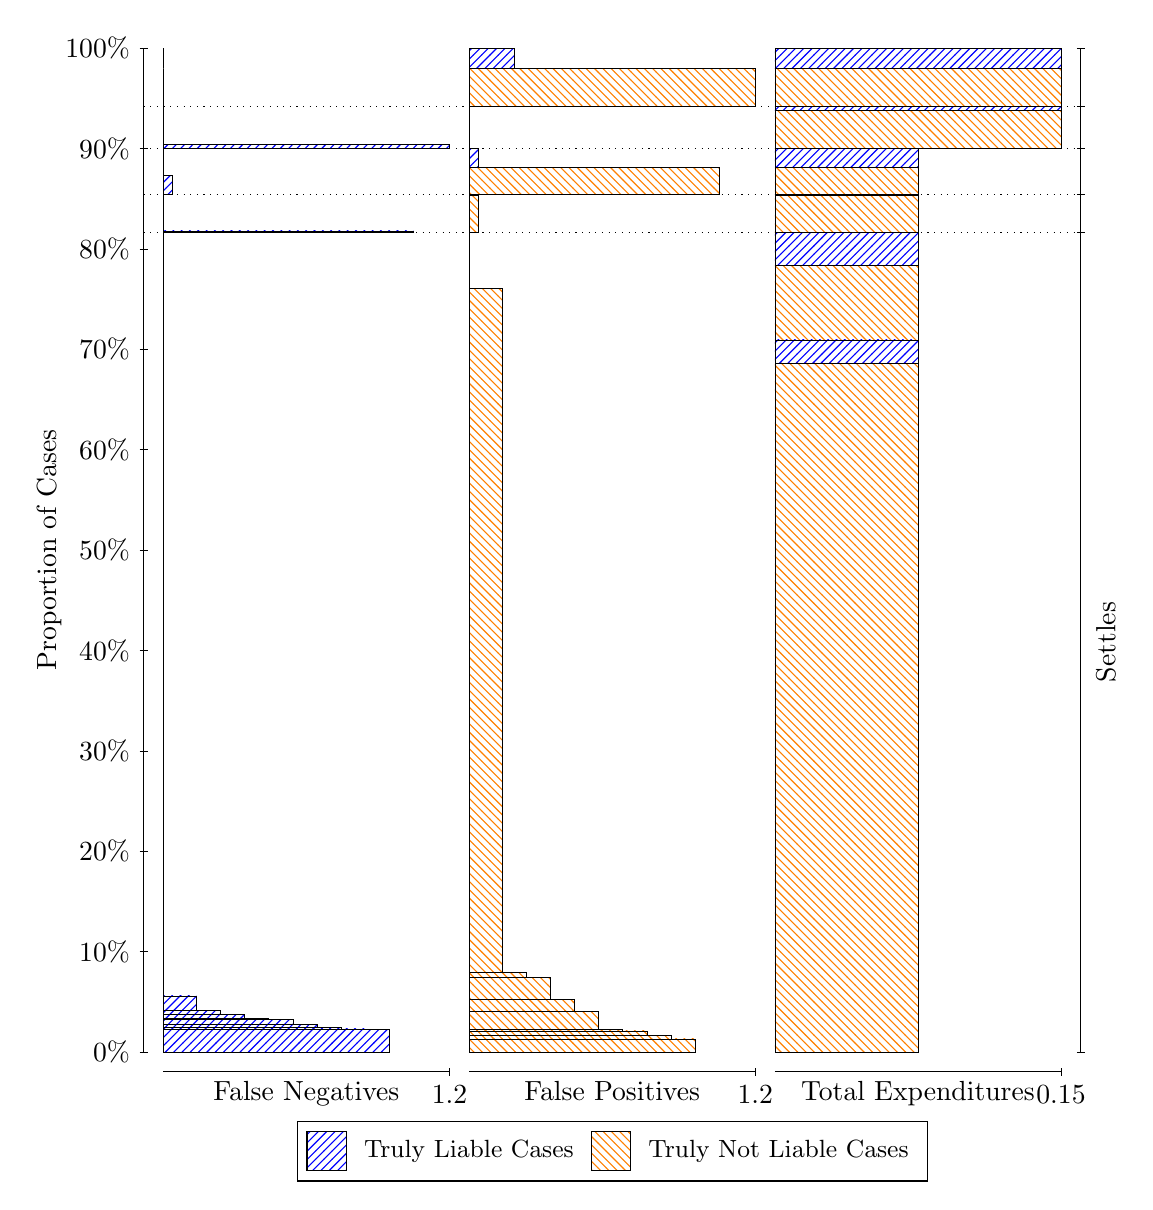
\begin{tikzpicture}
\draw[black, very thin] (1.5,1.75) -- (1.5,14.5);
\node[rotate=90, anchor=center] at (0.3, 8.125) {Proportion of Cases};
\draw[black, very thin] (1.45,1.75) -- (1.55,1.75);
\node[anchor=east] at (1.45, 1.75) {0\%};
\draw[black, very thin] (1.45,3.025) -- (1.55,3.025);
\node[anchor=east] at (1.45, 3.025) {10\%};
\draw[black, very thin] (1.45,4.3) -- (1.55,4.3);
\node[anchor=east] at (1.45, 4.3) {20\%};
\draw[black, very thin] (1.45,5.575) -- (1.55,5.575);
\node[anchor=east] at (1.45, 5.575) {30\%};
\draw[black, very thin] (1.45,6.85) -- (1.55,6.85);
\node[anchor=east] at (1.45, 6.85) {40\%};
\draw[black, very thin] (1.45,8.125) -- (1.55,8.125);
\node[anchor=east] at (1.45, 8.125) {50\%};
\draw[black, very thin] (1.45,9.4) -- (1.55,9.4);
\node[anchor=east] at (1.45, 9.4) {60\%};
\draw[black, very thin] (1.45,10.675) -- (1.55,10.675);
\node[anchor=east] at (1.45, 10.675) {70\%};
\draw[black, very thin] (1.45,11.95) -- (1.55,11.95);
\node[anchor=east] at (1.45, 11.95) {80\%};
\draw[black, very thin] (1.45,13.225) -- (1.55,13.225);
\node[anchor=east] at (1.45, 13.225) {90\%};
\draw[black, very thin] (1.45,14.5) -- (1.55,14.5);
\node[anchor=east] at (1.45, 14.5) {100\%};

\draw[black, very thin] (13.4,1.75) -- (13.4,14.5);
\draw[black, very thin] (13.35,1.75) -- (13.45,1.75);
\node[anchor=west] at (13.35, 1.75) {};
\draw[black, very thin] (13.35,12.162) -- (13.45,12.162);
\node[anchor=west] at (13.35, 12.162) {};
\draw[black, very thin] (13.35,12.643) -- (13.45,12.643);
\node[anchor=west] at (13.35, 12.643) {};
\draw[black, very thin] (13.35,13.223) -- (13.45,13.223);
\node[anchor=west] at (13.35, 13.223) {};
\draw[black, very thin] (13.35,13.763) -- (13.45,13.763);
\node[anchor=west] at (13.35, 13.763) {};
\draw[black, very thin] (13.35,14.5) -- (13.45,14.5);
\node[anchor=west] at (13.35, 14.5) {};

\draw[black, very thin, pattern color=blue, pattern=north east lines] (1.75,1.75) rectangle (4.6184,2.0327);
\draw[black, very thin, pattern color=blue, pattern=north east lines] (1.75,2.0327) rectangle (4.3125,2.0425);
\draw[black, very thin, pattern color=blue, pattern=north east lines] (1.75,2.0425) rectangle (4.0065,2.0664);
\draw[black, very thin, pattern color=blue, pattern=north east lines] (1.75,2.0664) rectangle (3.7005,2.1012);
\draw[black, very thin, pattern color=blue, pattern=north east lines] (1.75,2.1012) rectangle (3.3946,2.1638);
\draw[black, very thin, pattern color=blue, pattern=north east lines] (1.75,2.1638) rectangle (3.0886,2.1747);
\draw[black, very thin, pattern color=blue, pattern=north east lines] (1.75,2.1747) rectangle (2.7826,2.2244);
\draw[black, very thin, pattern color=blue, pattern=north east lines] (1.75,2.2244) rectangle (2.4767,2.2822);
\draw[black, very thin, pattern color=blue, pattern=north east lines] (1.75,2.2822) rectangle (2.1707,2.4616);
\draw[black, very thin, pattern color=orange, pattern=north west lines] (1.75,2.4616) rectangle (1.75,12.162);
\draw[black, very thin, pattern color=blue, pattern=north east lines] (1.75,12.162) rectangle (4.9244,12.178);
\draw[black, very thin, pattern color=orange, pattern=north west lines] (1.75,12.178) rectangle (1.75,12.643);
\draw[black, very thin, pattern color=blue, pattern=north east lines] (1.75,12.643) rectangle (1.8647,12.881);
\draw[black, very thin, pattern color=orange, pattern=north west lines] (1.75,12.881) rectangle (1.75,13.223);
\draw[black, very thin, pattern color=blue, pattern=north east lines] (1.75,13.223) rectangle (5.3833,13.275);
\draw[black, very thin, pattern color=orange, pattern=north west lines] (1.75,13.275) rectangle (1.75,13.763);
\draw[black, very thin, pattern color=orange, pattern=north west lines] (1.75,13.763) rectangle (1.75,14.243);
\draw[black, very thin, pattern color=blue, pattern=north east lines] (1.75,14.243) rectangle (1.75,14.5);
\draw[black, very thin, pattern color=orange, pattern=north west lines] (5.6333,1.75) rectangle (8.5018,1.9152);
\draw[black, very thin, pattern color=orange, pattern=north west lines] (5.6333,1.9152) rectangle (8.1958,1.9654);
\draw[black, very thin, pattern color=orange, pattern=north west lines] (5.6333,1.9654) rectangle (7.8898,2.0179);
\draw[black, very thin, pattern color=orange, pattern=north west lines] (5.6333,2.0179) rectangle (7.5839,2.0351);
\draw[black, very thin, pattern color=orange, pattern=north west lines] (5.6333,2.0351) rectangle (7.2779,2.2694);
\draw[black, very thin, pattern color=orange, pattern=north west lines] (5.6333,2.2694) rectangle (6.9719,2.2732);
\draw[black, very thin, pattern color=orange, pattern=north west lines] (5.6333,2.2732) rectangle (6.9719,2.4196);
\draw[black, very thin, pattern color=orange, pattern=north west lines] (5.6333,2.4196) rectangle (6.666,2.6998);
\draw[black, very thin, pattern color=orange, pattern=north west lines] (5.6333,2.6998) rectangle (6.36,2.7576);
\draw[black, very thin, pattern color=orange, pattern=north west lines] (5.6333,2.7576) rectangle (6.054,11.45);
\draw[black, very thin, pattern color=blue, pattern=north east lines] (5.6333,11.45) rectangle (5.6333,12.162);
\draw[black, very thin, pattern color=orange, pattern=north west lines] (5.6333,12.162) rectangle (5.7481,12.627);
\draw[black, very thin, pattern color=blue, pattern=north east lines] (5.6333,12.627) rectangle (5.6333,12.643);
\draw[black, very thin, pattern color=orange, pattern=north west lines] (5.6333,12.643) rectangle (8.8077,12.985);
\draw[black, very thin, pattern color=blue, pattern=north east lines] (5.6333,12.985) rectangle (5.7481,13.223);
\draw[black, very thin, pattern color=orange, pattern=north west lines] (5.6333,13.223) rectangle (5.6333,13.711);
\draw[black, very thin, pattern color=blue, pattern=north east lines] (5.6333,13.711) rectangle (5.6333,13.763);
\draw[black, very thin, pattern color=orange, pattern=north west lines] (5.6333,13.763) rectangle (9.2667,14.243);
\draw[black, very thin, pattern color=blue, pattern=north east lines] (5.6333,14.243) rectangle (6.207,14.5);
\draw[black, very thin, pattern color=orange, pattern=north west lines] (9.5167,1.75) rectangle (11.333,10.5);
\draw[black, very thin, pattern color=blue, pattern=north east lines] (9.5167,10.5) rectangle (11.333,10.793);
\draw[black, very thin, pattern color=orange, pattern=north west lines] (9.5167,10.793) rectangle (11.333,11.743);
\draw[black, very thin, pattern color=blue, pattern=north east lines] (9.5167,11.743) rectangle (11.333,12.162);
\draw[black, very thin, pattern color=orange, pattern=north west lines] (9.5167,12.162) rectangle (11.333,12.627);
\draw[black, very thin, pattern color=blue, pattern=north east lines] (9.5167,12.627) rectangle (11.333,12.643);
\draw[black, very thin, pattern color=orange, pattern=north west lines] (9.5167,12.643) rectangle (11.333,12.985);
\draw[black, very thin, pattern color=blue, pattern=north east lines] (9.5167,12.985) rectangle (11.333,13.223);
\draw[black, very thin, pattern color=orange, pattern=north west lines] (9.5167,13.223) rectangle (13.15,13.711);
\draw[black, very thin, pattern color=blue, pattern=north east lines] (9.5167,13.711) rectangle (13.15,13.763);
\draw[black, very thin, pattern color=orange, pattern=north west lines] (9.5167,13.763) rectangle (13.15,14.243);
\draw[black, very thin, pattern color=blue, pattern=north east lines] (9.5167,14.243) rectangle (13.15,14.5);
\draw[black, dotted] (1.5,12.162) -- (13.4,12.162);
\draw[black, dotted] (1.5,12.643) -- (13.4,12.643);
\draw[black, dotted] (1.5,13.223) -- (13.4,13.223);
\draw[black, dotted] (1.5,13.763) -- (13.4,13.763);
\draw[black, very thin] (1.75,1.5) -- (5.3833,1.5);
\node[anchor=north] at (3.5667, 1.5) {False Negatives};
\draw[black, very thin] (5.3833,1.45) -- (5.3833,1.55);
\node[anchor=north] at (5.3833, 1.45) {1.2};

\draw[black, very thin] (5.6333,1.5) -- (9.2667,1.5);
\node[anchor=north] at (7.45, 1.5) {False Positives};
\draw[black, very thin] (9.2667,1.45) -- (9.2667,1.55);
\node[anchor=north] at (9.2667, 1.45) {1.2};

\draw[black, very thin] (9.5167,1.5) -- (13.15,1.5);
\node[anchor=north] at (11.333, 1.5) {Total Expenditures};
\draw[black, very thin] (13.15,1.45) -- (13.15,1.55);
\node[anchor=north] at (13.15, 1.45) {0.15};

\node[black, centered, rotate=90] at (13.72, 6.9559) {Settles};





\draw (7.449999999999999,1.5) node[draw=none] (baseCoordinate) {};
\begin{scope}[align=center]
        \matrix[scale=0.5, draw=black, below=0.5cm of baseCoordinate, nodes={draw}, column sep=0.1cm]{
            \node[rectangle, draw, minimum width=0.5cm, minimum height=0.5cm, pattern=north east lines, pattern color=blue] {}; &
            \node[draw=none, font=\small] (B) {Truly Liable Cases}; &
            \node[rectangle, draw, minimum width=0.5cm, minimum height=0.5cm, pattern=north west lines, pattern color=orange] {}; &
            \node[draw=none, font=\small] (B) {Truly Not Liable Cases}; \\
            };
\end{scope}

\end{tikzpicture}
\end{document}